% Created 2023-11-13 lun 12:07
% Intended LaTeX compiler: pdflatex
\documentclass[aspectratio=169, usenames,svgnames,dvipsnames]{beamer}
\usepackage[utf8]{inputenc}
\usepackage[T1]{fontenc}
\usepackage{graphicx}
\usepackage{grffile}
\usepackage{longtable}
\usepackage{wrapfig}
\usepackage{rotating}
\usepackage[normalem]{ulem}
\usepackage{amsmath}
\usepackage{textcomp}
\usepackage{amssymb}
\usepackage{capt-of}
\usepackage{hyperref}
\usepackage{color}
\usepackage{listings}
\usepackage{mathpazo}
\usepackage[spanish]{babel}
\usepackage{gensymb}
\usepackage{amsmath}
\usepackage{diffcoeff}
\usepackage{steinmetz}
\usepackage{mathtools}
\bibliographystyle{plain}
\usepackage{siunitx}
\sisetup{output-decimal-marker={,}}
\DeclareSIUnit{\watthour}{Wh}
\hypersetup{colorlinks=true, linkcolor=Blue, urlcolor=Blue}
\usepackage[symbol, perpage]{footmisc}
\newcommand{\laplace}[1]{\mathbf{#1}(\mathbf{s})}
\newcommand{\slp}{\mathbf{s}}
\newcommand{\fasor}[1]{\mathbf{#1}(\omega)}
\newcommand{\atan}{\mathrm{atan}}
\parskip=5pt
\usetheme{Boadilla}
\usecolortheme{rose}
\usefonttheme{serif}
\author{Oscar Perpiñán Lamigueiro}
\date{}
\title{Sistemas Trifásicos}
\setbeamercolor{alerted text}{fg=blue!50!black} \setbeamerfont{alerted text}{series=\bfseries}
\AtBeginSubsection[]{\begin{frame}[plain]\tableofcontents[currentsubsection,sectionstyle=show/shaded,subsectionstyle=show/shaded/hide]\end{frame}}
\AtBeginSection[]{\begin{frame}[plain]\tableofcontents[currentsection,hideallsubsections]\end{frame}}
\beamertemplatenavigationsymbolsempty
\setbeamertemplate{footline}[frame number]
\setbeamertemplate{itemize items}[triangle]
\setbeamertemplate{enumerate items}[circle]
\setbeamertemplate{section in toc}[circle]
\setbeamertemplate{subsection in toc}[circle]
\hypersetup{
 pdfauthor={Oscar Perpiñán Lamigueiro},
 pdftitle={Sistemas Trifásicos},
 pdfkeywords={},
 pdfsubject={},
 pdfcreator={Emacs 29.1 (Org mode 9.4.6)}, 
 pdflang={Spanish}}
\begin{document}

\maketitle

\section{Introducción}
\label{sec:orgfc846af}

\begin{frame}[label={sec:orgd7567c0},plain]{}
\begin{center}
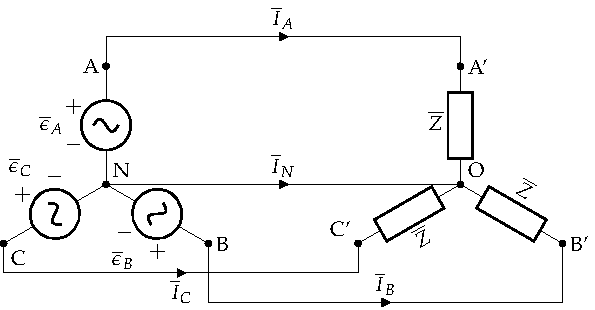
\includegraphics[width=.9\linewidth]{../figs/EstrellaEquilibrado.pdf}
\end{center}
\end{frame}

\begin{frame}[label={sec:org909009b}]{Motivación de los sistemas trifásicos}
\begin{itemize}
\item En un sistema trifásico la potencia instantánea es constante, evitando vibraciones y esfuerzos en las máquinas. (\emph{La potencia instantánea de un sistema monofásico es pulsante.})

\item La masa de conductor necesaria en un sistema trifásico es un 25\% inferior que en un monofásico para transportar la misma potencia.
\end{itemize}
\end{frame}

\begin{frame}[label={sec:org4e454ae}]{Ondas Trifásicas}
\begin{center}
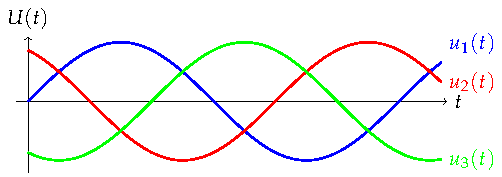
\includegraphics[width=.9\linewidth]{../figs/TensionesTrifasica.pdf}
\end{center}

\begin{align*}
  u_1(t) &= U_0 \sin(\omega t)\\
  u_2(t) &= U_0 \sin(\omega t + 2\pi/3)\\
  u_3(t) &= U_0 \sin(\omega t - 2\pi/3)
\end{align*}
\end{frame}

\begin{frame}[label={sec:org713a81d}]{Fasores de un sistema trifásico}
\begin{center}
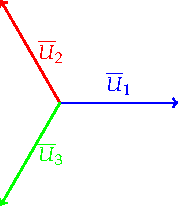
\includegraphics[height=0.5\textheight]{../figs/FasoresTrifasica.pdf}
\end{center}

\begin{align*}
  \overline{U}_1 &= U\phase{0}\\
  \overline{U}_2 &= U\phase{2\pi/3}\\
  \overline{U}_3 &= U\phase{-2\pi/3}
\end{align*}
\end{frame}

\section{Generadores}
\label{sec:org1f51dc4}
\begin{frame}[label={sec:orgabb8a52}]{Conexión}
\begin{center}
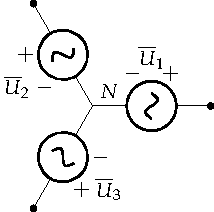
\includegraphics[height=0.5\textheight]{../figs/GeneradoresTrifasica.pdf}
\end{center}

\begin{columns}
\begin{column}{0.5\columnwidth}
\begin{align*}
  u_1(t) &= U_0 \sin(\omega t)\\
  u_2(t) &= U_0 \sin(\omega t + 2\pi/3)\\
  u_3(t) &= U_0 \sin(\omega t - 2\pi/3)
\end{align*}
\end{column}

\begin{column}{0.5\columnwidth}
\begin{align*}
  \overline{U}_1 &= U\phase{0}\\
  \overline{U}_2 &= U\phase{2\pi/3}\\
  \overline{U}_3 &= U\phase{-2\pi/3}
\end{align*}
\end{column}
\end{columns}
\end{frame}

\begin{frame}[label={sec:org7bb286b}]{Las tensiones suman 0}
\begin{center}
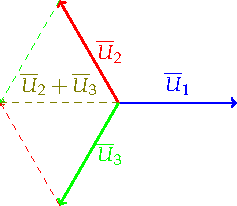
\includegraphics[height=0.6\textheight]{../figs/FasoresSumaCero.pdf}
\end{center}

\[
\boxed{\overline{U}_1 + \overline{U}_2 + \overline{U}_3 = 0}
\]
\end{frame}

\begin{frame}[label={sec:orgc82d561}]{Las tensiones suman 0}
\begin{center}
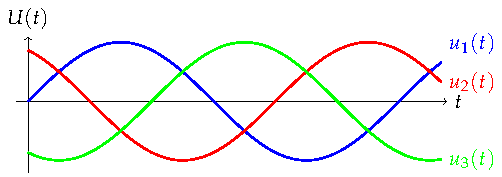
\includegraphics[width=.9\linewidth]{../figs/TensionesTrifasica.pdf}
\end{center}

\[
\boxed{u_1(t) + u_2(t) + u_3(t) = 0}
\]
\end{frame}


\begin{frame}[label={sec:org5c008fd}]{Tensiones de Fase y Línea}
\begin{columns}
\begin{column}{0.4\columnwidth}
\begin{center}
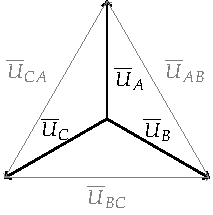
\includegraphics[height=0.4\textheight]{../figs/FasoresTrifasica_ABC.pdf}
\end{center}
\end{column}

\begin{column}{0.6\columnwidth}
Tensiones de \alert{Fase}: \(U_A\), \(U_B\), \(U_C\)

Tensiones de \alert{Línea}: \(U_{AB}\), \(U_{BC}\), \(U_{CA}\)
\end{column}
\end{columns}

     \begin{align*}
       \overline{U}_{AB} &= \overline{U}_A - \overline{U}_B\\
       \overline{U}_{BC} &= \overline{U}_B - \overline{U}_C\\
       \overline{U}_{CA} &= \overline{U}_C - \overline{U}_A\\
\cline{1-2}
       \overline{U}_{AB} + \overline{U}_{BC} + \overline{U}_{CA} &= 0     \end{align*}
\end{frame}

\begin{frame}[label={sec:orgebfa50f}]{Tensiones de Fase y Línea}
\begin{columns}
\begin{column}{0.5\columnwidth}
\begin{align*}
  \overline{U}_A &= U_f\phase{\theta_f}\\
  \overline{U}_B &= U_f\phase{\theta_f - \ang{120}}
\end{align*}

\begin{align*}
\overline{U}_{AB} &= \overline{U}_A - \overline{U}_B = \\
		  &= U_f\phase{\theta_f} - U_f\phase{\theta_f - \ang{120}} = \\
		  &= U_f\phase{\theta_f} + U_f\phase{\theta_f + \ang{60}}\\
		  &= 2 \cdot U_f \cdot \cos(30) \phase{\theta_f + \ang{30}} = \\
  &= \sqrt{3} U_f \phase{\theta_f + \ang{30}}
\end{align*}
\end{column}

\begin{column}{0.5\columnwidth}
\begin{center}
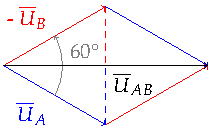
\includegraphics[width=.9\linewidth]{../figs/FasoresFaseLinea.pdf}
\end{center}

\[
  \boxed{
    \begin{array}{l}
      U = \sqrt{3}\cdot U_f\\
      \theta_l = \theta_f + \ang{30}\\
    \end{array}
  }
\]
\end{column}
\end{columns}
\end{frame}
\begin{frame}[label={sec:org2afafe4}]{Secuencia de Fases}
\begin{itemize}
\item Sentido en el que ocurren los máximos de cada fase.
\item Secuencia de Fases Directa (\alert{SFD}): ABC
\end{itemize}
\begin{center}
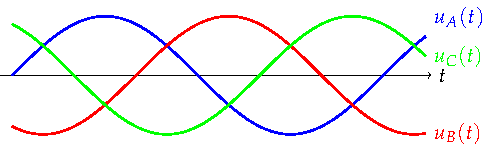
\includegraphics[height=0.3\textheight]{../figs/TensionesTrifasica_ABC.pdf}
\end{center}
\begin{itemize}
\item Secuencia de Fases Inversa (\alert{SFI}): ACB
\end{itemize}
\begin{center}
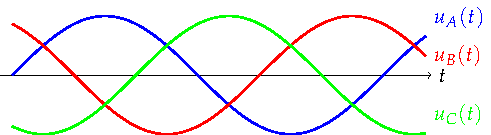
\includegraphics[height=0.3\textheight]{../figs/TensionesTrifasica_ACB.pdf}
\end{center}
\end{frame}

\begin{frame}[label={sec:orgc9a86a2}]{Secuencia de Fases Directa (SFD)}
\begin{center}
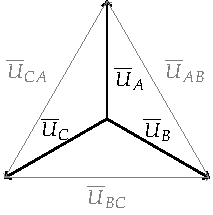
\includegraphics[height=0.45\textheight]{../figs/FasoresTrifasica_ABC.pdf}
\end{center}

\begin{columns}
\begin{column}{0.4\columnwidth}
\begin{align*}
  \overline{U}_A &= \frac{U}{\sqrt{3}}\phase{{\color{blue}\ang{90}}}\\
  \overline{U}_B &= \frac{U}{\sqrt{3}}\phase{\ang{-30}}\\
  \overline{U}_C &= \frac{U}{\sqrt{3}}\phase{\ang{-150}}
\end{align*}
\end{column}
\begin{column}{0.2\columnwidth}
\begin{center}
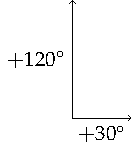
\includegraphics[width=.9\linewidth]{../figs/ReglaSFD.pdf}
\end{center}
\end{column}

\begin{column}{0.4\columnwidth}
\begin{align*}
  \overline{U}_{AB} &= U\phase{\ang{120}}\\
  \overline{U}_{BC} &= U\phase{{\color{blue}\ang{0}}}\\
  \overline{U}_{CA} &= U\phase{\ang{-120}}
\end{align*}
\end{column}
\end{columns}
\end{frame}


\begin{frame}[label={sec:org81f7fbf}]{Secuencia de Fases Inversa (SFI)}
\begin{center}
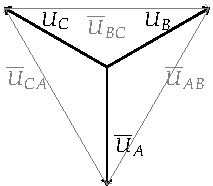
\includegraphics[height=0.45\textheight]{../figs/FasoresTrifasica_ACB.pdf}
\end{center}
\begin{columns}
\begin{column}{0.4\columnwidth}
\begin{align*}
  \overline{U}_A &= \frac{U}{\sqrt{3}}\phase{{\color{blue}\ang{-90}}}\\
  \overline{U}_B &= \frac{U}{\sqrt{3}}\phase{\ang{30}}\\
  \overline{U}_C &= \frac{U}{\sqrt{3}}\phase{\ang{150}}
\end{align*}
\end{column}

\begin{column}{0.2\columnwidth}
\begin{center}
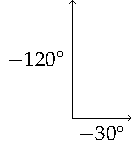
\includegraphics[width=.9\linewidth]{../figs/ReglaSFI.pdf}
\end{center}
\end{column}
\begin{column}{0.4\columnwidth}
\begin{align*}
  \overline{U}_{AB} &= U\phase{\ang{-120}}\\
  \overline{U}_{BC} &= U\phase{{\color{blue}\ang{0}}}\\
  \overline{U}_{CA} &= U\phase{\ang{120}}
\end{align*}
\end{column}
\end{columns}
\end{frame}
\section{Receptores}
\label{sec:orge50d969}
\begin{frame}[label={sec:org8244150}]{Tipos de Receptores}
\begin{block}{Conexión}
\begin{itemize}
\item \alert{Estrella} (punto común) Y
\item \alert{Triángulo} \(\triangle\)
\end{itemize}
\end{block}

\begin{block}{Impedancias}
\begin{itemize}
\item \alert{Equilibrado} (las tres impedancias son idénticas en módulo \alert{y} fase).
\item \alert{Desequilibrado}
\end{itemize}
\end{block}
\end{frame}


\subsection{Receptores Equilibrados}
\label{sec:org816d14a}

\begin{frame}[label={sec:org97666d2}]{Receptor en Estrella Equilibrado}
\begin{center}
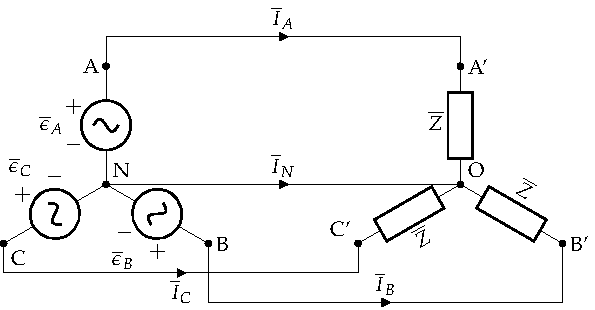
\includegraphics[width=.9\linewidth]{../figs/EstrellaEquilibrado.pdf}
\end{center}
\end{frame}

\begin{frame}[label={sec:org5b6c941}]{Receptor en Estrella Equilibrado}
\begin{columns}
\begin{column}{0.5\columnwidth}
\begin{center}
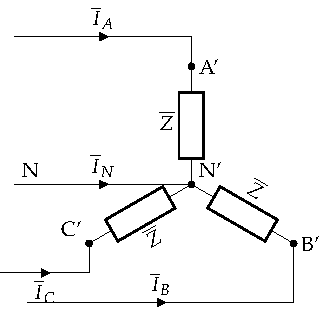
\includegraphics[width=.9\linewidth]{../figs/EstrellaEquilibrado_Receptor.pdf}
\end{center}
\end{column}

\begin{column}{0.5\columnwidth}
\begin{align*}
  \overline{I}_A &= \frac{\overline{U}_A}{\overline{Z}} = \frac{U_f}{Z}\phase{\ang{\pm 90} - \theta} \\
  \overline{I}_B &= \frac{\overline{U}_B}{\overline{Z}} = \frac{U_f}{Z}\phase{\ang{\mp 30} - \theta}\\
  \overline{I}_C &= \frac{\overline{U}_C}{\overline{Z}} = \frac{U_f}{Z}\phase{\ang{\mp 150} - \theta}
\end{align*}


\[
  \boxed{|\overline{I}_A| = |\overline{I}_B| = |\overline{I}_C| = \frac{U_f}{Z}}
\]

\[
  \overline{I}_A  + \overline{I}_B + \overline{I}_C + \overline{I}_N = 0
\]
\[
   \overline{I}_A  + \overline{I}_B + \overline{I}_C  = 0 \rightarrow \boxed{\overline{I}_N = 0}
\]
\end{column}
\end{columns}
\end{frame}
\begin{frame}[label={sec:org9e952bd}]{Receptor en Estrella Equilibrado}
\begin{center}
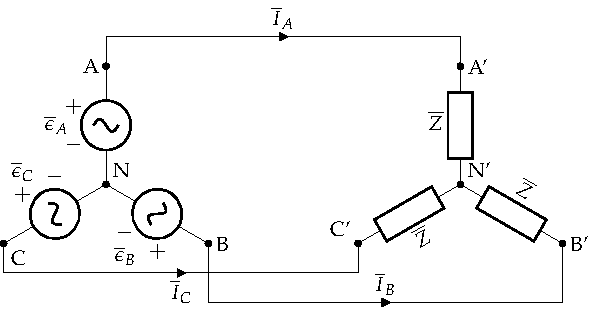
\includegraphics[width=.9\linewidth]{../figs/EstrellaEquilibrado_SinNeutro.pdf}
\end{center}
\end{frame}

\begin{frame}[label={sec:org113d8d1}]{Receptor en Triángulo Equilibrado}
\begin{center}
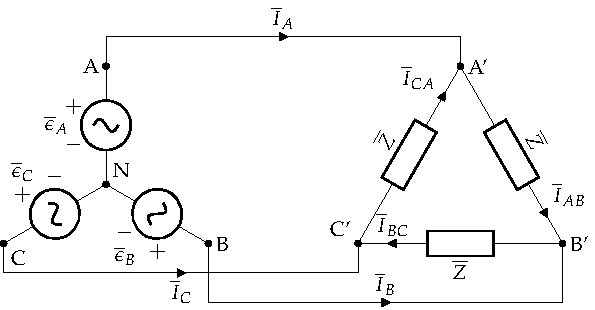
\includegraphics[width=.9\linewidth]{../figs/TrianguloEquilibrado.pdf}
\end{center}
\end{frame}

\begin{frame}[label={sec:orgabfad9d}]{Receptor en Triángulo Equilibrado}
\begin{columns}
\begin{column}{0.5\columnwidth}
\begin{center}
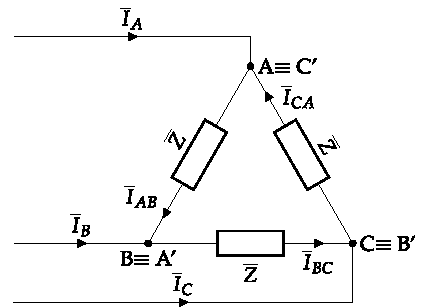
\includegraphics[width=.9\linewidth]{../figs/TrianguloEquilibrado_Receptor.pdf}
\end{center}
\end{column}

\begin{column}{0.5\columnwidth}
\begin{align*}
  \overline{I}_{AB} &= \frac{\overline{U}_{AB}}{\overline{Z}} = \frac{U}{Z}\phase{\ang{\pm 120} - \theta} \\
  \overline{I}_{BC} &= \frac{\overline{U}_{BC}}{\overline{Z}} = \frac{U}{Z}\phase{0 - \theta}\\
  \overline{I}_{CA} &= \frac{\overline{U}_{CA}}{\overline{Z}} = \frac{U}{Z}\phase{\ang{\mp 120} - \theta}
\end{align*}

\[
   \overline{I}_{AB}  + \overline{I}_{BC} + \overline{I}_{CA}  = 0 
\]

Corriente de Fase:
\[
  \boxed{I_f = |\overline{I}_{AB}| = |\overline{I}_{BC}| = |\overline{I}_{CA}| = \frac{U}{Z}}
\]
\end{column}
\end{columns}
\end{frame}


\begin{frame}[label={sec:org6ea97b6}]{Receptor en Triángulo Equilibrado}
\begin{columns}
\begin{column}{0.5\columnwidth}
\begin{center}
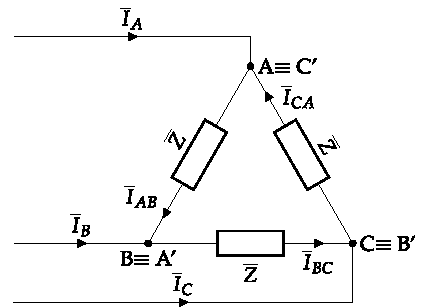
\includegraphics[width=.9\linewidth]{../figs/TrianguloEquilibrado_Receptor.pdf}
\end{center}
\end{column}

\begin{column}{0.5\columnwidth}
\begin{align*}
  \overline{I}_A &= \overline{I}_{AB} - \overline{I}_{CA} = \sqrt{3} \cdot \frac{U}{Z}\phase{\ang{\pm 90} - \theta}\\
  \overline{I}_B &= \overline{I}_{BC} - \overline{I}_{AB} = \sqrt{3} \cdot \frac{U}{Z}\phase{\ang{\mp 30} - \theta}\\
  \overline{I}_C &= \overline{I}_{CA} - \overline{I}_{BC} = \sqrt{3} \cdot \frac{U}{Z}\phase{\ang{\mp 150} - \theta}\\
\end{align*}

Corriente de Línea:
\[
  \boxed{I = |\overline{I}_A| = |\overline{I}_B| = |\overline{I}_C| = \sqrt{3} \cdot \frac{U}{Z}}
\]

\[
  \boxed{I = \sqrt{3} \cdot I_f}
\]
\end{column}
\end{columns}
\end{frame}


\subsection{Receptores Desequilibrados}
\label{sec:orga263201}

\begin{frame}[label={sec:org53212b1}]{Receptor en Estrella Desequilibrado con Neutro}
\begin{center}
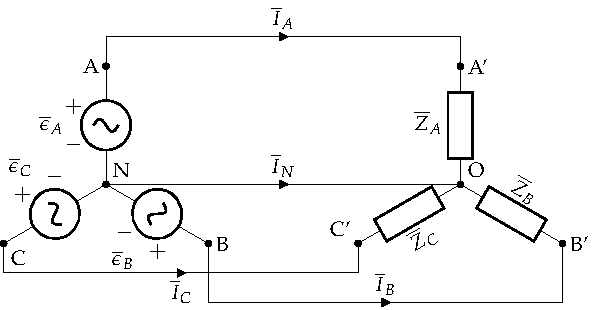
\includegraphics[width=.9\linewidth]{../figs/EstrellaDesequilibrado.pdf}
\end{center}
\end{frame}

\begin{frame}[label={sec:org03e2e59}]{Receptor en Estrella Desequilibrado con Neutro}
\begin{columns}
\begin{column}{0.5\columnwidth}
\begin{center}
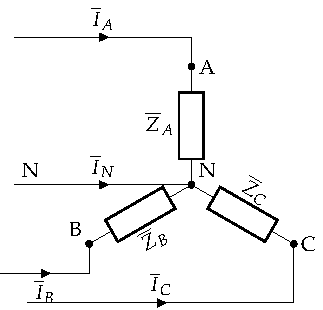
\includegraphics[width=.9\linewidth]{../figs/EstrellaDesequilibrado_Receptor.pdf}
\end{center}
\end{column}

\begin{column}{0.5\columnwidth}
\begin{align*}
  \overline{I}_A &= \frac{\overline{U}_A}{\overline{Z}_A}\\
  \overline{I}_B &= \frac{\overline{U}_B}{\overline{Z}_B}\\
  \overline{I}_C &= \frac{\overline{U}_C}{\overline{Z}_C}
\end{align*}

\[
  \overline{I}_A  + \overline{I}_B + \overline{I}_C + \overline{I}_N = 0
\]
\[
   \overline{I}_A  + \overline{I}_B + \overline{I}_C  \neq 0 \rightarrow \boxed{\overline{I}_N \neq 0}
\]
\end{column}
\end{columns}
\end{frame}

\begin{frame}[label={sec:org8edb0e2}]{Receptor en Estrella Desequilibrado sin Neutro}
\begin{center}
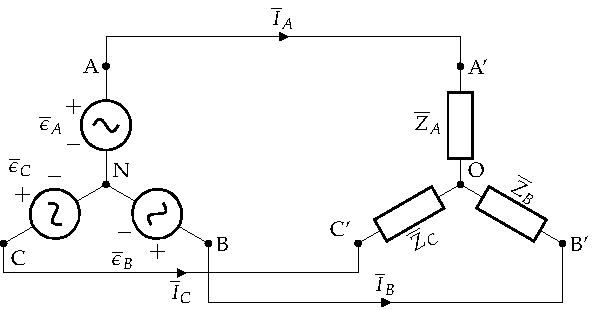
\includegraphics[width=.9\linewidth]{../figs/EstrellaDesequilibrado_SinNeutro.pdf}
\end{center}

\[
\overline{U}_N \neq \overline{U}_{O}
\]
\end{frame}
\begin{frame}[label={sec:org7c23148}]{Receptor en Estrella con Carga Monofásica}
\begin{center}
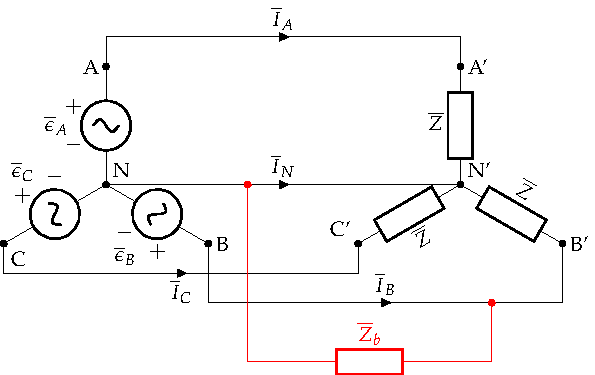
\includegraphics[height=0.9\textheight]{../figs/Estrella_CargaMonofasica.pdf}
\end{center}
\end{frame}
\begin{frame}[label={sec:org32aae40}]{Receptor en Triángulo Desequilibrado}
\begin{center}
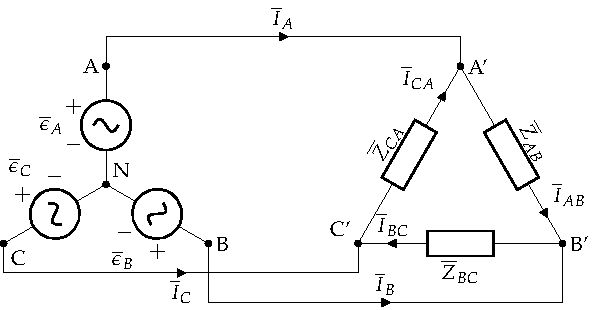
\includegraphics[height=0.9\textheight]{../figs/TrianguloDesequilibrado.pdf}
\end{center}
\end{frame}

\begin{frame}[label={sec:orgdda6f28}]{Receptor en Triángulo Desequilibrado}
\begin{columns}
\begin{column}{0.6\columnwidth}
\begin{center}
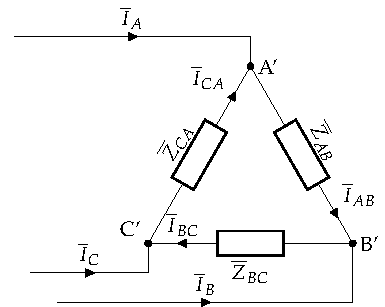
\includegraphics[width=.9\linewidth]{../figs/TrianguloDesequilibrado_Receptor.pdf}
\end{center}
\end{column}

\begin{column}{0.4\columnwidth}
\begin{align*}
  \overline{I}_{AB} &= \frac{\overline{U}_{AB}}{\overline{Z}_{AB}}\\
  \overline{I}_{BC} &= \frac{\overline{U}_{BC}}{\overline{Z}_{BC}}\\
  \overline{I}_{CA} &= \frac{\overline{U}_{CA}}{\overline{Z}_{CA}}
\end{align*}

\begin{align*}
  \overline{I}_A &= \overline{I}_{AB} - \overline{I}_{CA}\\
  \overline{I}_B &= \overline{I}_{BC} - \overline{I}_{AB}\\
  \overline{I}_C &= \overline{I}_{CA} - \overline{I}_{BC}\\
\end{align*}
\end{column}
\end{columns}
\end{frame}


\section{Potencia en Sistemas Trifásicos}
\label{sec:org2da38af}


\subsection{Cálculo de potencia}
\label{sec:org15b8c8a}
\begin{frame}[label={sec:orgb3bf385}]{Receptor en Estrella Equilibrado}
\begin{columns}
\begin{column}{0.5\columnwidth}
\begin{center}
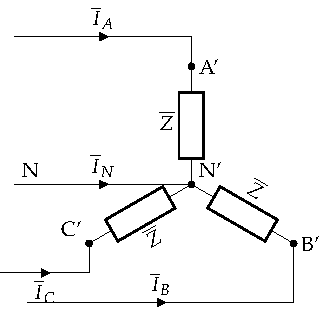
\includegraphics[width=.9\linewidth]{../figs/EstrellaEquilibrado_Receptor.pdf}
\end{center}
\end{column}

\begin{column}{0.5\columnwidth}
\begin{align*}
  P = 3 \cdot P_Z &= 3 \cdot U_Z I_Z \cos(\theta)\\
  Q = 3 \cdot Q_Z &= 3 \cdot U_Z I_Z \sin(\theta)
\end{align*}

\begin{align*}
  I_Z &= I\\
  U_Z &= U_F
\end{align*}


\begin{align*}
  P &= 3 U_F I \cos(\theta) = \sqrt{3} U I \cos(\theta)\\
  Q &= 3 U_F I \sin(\theta) = \sqrt{3} U I \sin(\theta)\\
  S &= \sqrt{P^2 + Q^2} =  \sqrt{3} U I
\end{align*}
\end{column}
\end{columns}
\end{frame}


\begin{frame}[label={sec:orgd1a9761}]{Receptor en Triángulo Equilibrado}
\begin{columns}
\begin{column}{0.5\columnwidth}
\begin{center}
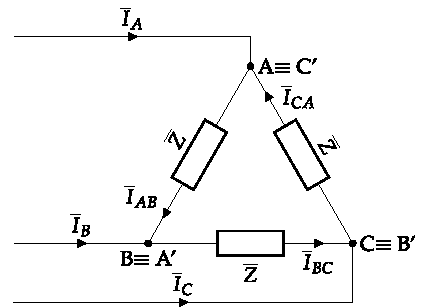
\includegraphics[width=.9\linewidth]{../figs/TrianguloEquilibrado_Receptor.pdf}
\end{center}
\end{column}

\begin{column}{0.5\columnwidth}
\begin{align*}
  P = 3 \cdot P_Z &= 3 \cdot U_Z I_Z \cos(\theta)\\
  Q = 3 \cdot Q_Z &= 3 \cdot U_Z I_Z \sin(\theta)
\end{align*}

\begin{align*}
  I_Z &= I_F\\
  U_Z &= U
\end{align*}


\begin{align*}
  P &= 3 U I_F \cos(\theta) = \sqrt{3} U I \cos(\theta)\\
  Q &= 3 U I_F \sin(\theta) = \sqrt{3} U I \sin(\theta)\\
  S &= \sqrt{P^2 + Q^2} =  \sqrt{3} U I
\end{align*}
\end{column}
\end{columns}
\end{frame}

\begin{frame}[label={sec:orgc248fdd}]{Receptor en Estrella Desequilibrado}
\begin{columns}
\begin{column}{0.5\columnwidth}
\begin{center}
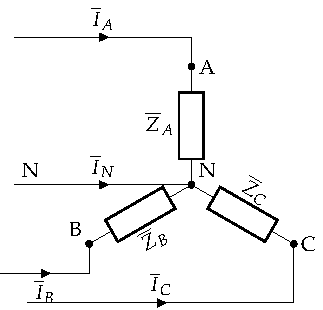
\includegraphics[width=.9\linewidth]{../figs/EstrellaDesequilibrado_Receptor.pdf}
\end{center}
\end{column}

\begin{column}{0.5\columnwidth}
\begin{align*}
  P &= P_A + P_B + P_C\\
  Q &= Q_A + Q_B + Q_C\\
  \overline{S} &= P + jQ
\end{align*}
\end{column}
\end{columns}
\end{frame}

\begin{frame}[label={sec:org54935a5}]{Receptor en Triángulo Desequilibrado}
\begin{columns}
\begin{column}{0.6\columnwidth}
\begin{center}
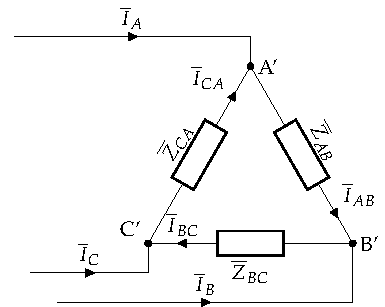
\includegraphics[width=.9\linewidth]{../figs/TrianguloDesequilibrado_Receptor.pdf}
\end{center}
\end{column}

\begin{column}{0.4\columnwidth}
\begin{align*}
  P &= P_{AB} + P_{BC} + P_{CA}\\
  Q &= Q_{AB} + Q_{BC} + Q_{CA}\\
  \overline{S} &= P + jQ
\end{align*}
\end{column}
\end{columns}
\end{frame}

\subsection{Medida de Potencia en Sistemas Trifásicos}
\label{sec:org0d737c1}
\begin{frame}[label={sec:org5ced2d3}]{Recordatorio: vatímetro}
\begin{center}
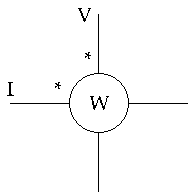
\includegraphics[height=0.6\textheight]{../figs/vatimetro.pdf}
\end{center}

\alert{Vatímetro}: equipo de medida de 4 terminales (1 par para tensión, 1 par para corriente)

\[
  \boxed{W = \Re(\overline{U} \cdot \overline{I}^*)}
\]
\end{frame}
\begin{frame}[label={sec:orgfca6e37}]{Sistema de 4 Hilos}
\begin{columns}
\begin{column}{0.7\columnwidth}
\begin{center}
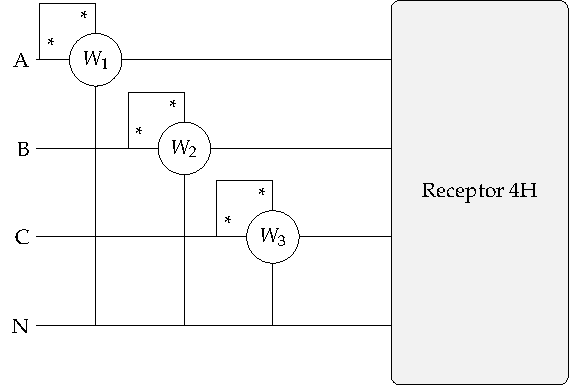
\includegraphics[height=0.85\textheight]{../figs/Potencia4H.pdf}
\end{center}
\end{column}

\begin{column}{0.3\columnwidth}
\begin{align*}
  W_1 &= \Re(\overline{U}_A \cdot \overline{I}_A^*) = P_A\\
  W_2 &= \Re(\overline{U}_B \cdot \overline{I}_B^*) = P_B\\
  W_3 &= \Re(\overline{U}_C \cdot \overline{I}_C^*) = P_C\\
\end{align*}

\[
  \boxed{P = W_1 + W_2 + W_3}
\]
\end{column}
\end{columns}
\end{frame}


\begin{frame}[label={sec:org7898931}]{Sistema de 4 Hilos Equilibrado}
\begin{columns}
\begin{column}{0.6\columnwidth}
\begin{center}
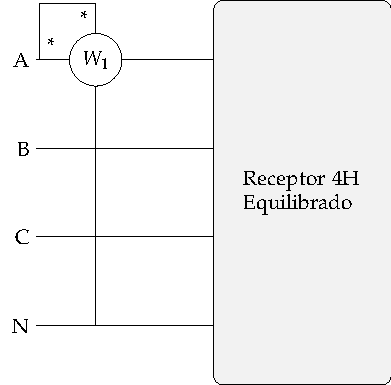
\includegraphics[height=0.85\textheight]{../figs/Potencia4H_Equilibrado.pdf}
\end{center}
\end{column}

\begin{column}{0.4\columnwidth}
\[
  P_A = P_B = P_C
\]

\[
\boxed{P = 3 \cdot W_1}
\]
\end{column}
\end{columns}
\end{frame}


\begin{frame}[label={sec:org021afe1}]{Sistema de 3 Hilos}
\begin{columns}
\begin{column}{0.7\columnwidth}
\begin{center}
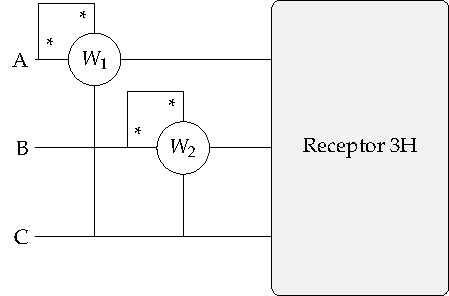
\includegraphics[width=.9\linewidth]{../figs/Potencia3H.pdf}
\end{center}
\end{column}

\begin{column}{0.3\columnwidth}
Montaje de Aron
\begin{align*}
  W_1 &= \Re(\overline{U}_{AC} \cdot \overline{I}^*_A)\\
  W_2 &= \Re(\overline{U}_{BC} \cdot \overline{I}^*_B)\\
  W_1 + W_2 &= ?
\end{align*}
\end{column}
\end{columns}
\end{frame}


\begin{frame}[label={sec:orgda61f37}]{Sistema de 3 Hilos}
Desarrollamos las dos expresiones usando corrientes de fase y obviando el operador \(\Re\):
\begin{align*}
  \overline{U}_{AC} \cdot \overline{I}^*_A &=   \overline{U}_{AC} \cdot (\overline{I}^*_{AB} - \overline{I}^*_{CA})\\
  \overline{U}_{BC} \cdot \overline{I}^*_B &=   \overline{U}_{BC} \cdot (\overline{I}^*_{BC} - \overline{I}^*_{AB})
\end{align*}
Sumamos las dos expresiones:
    \[
      \overline{U}_{AC} \cdot \overline{I}^*_A + \overline{U}_{BC} \cdot \overline{I}^*_B =   \overline{U}_{AC} \cdot \overline{I}^*_{AB} - \overline{U}_{AC} \cdot \overline{I}^*_{CA} + \overline{U}_{BC} \cdot \overline{I}^*_{BC} - \overline{U}_{BC} \cdot \overline{I}^*_{AB}
\]
Y agrupamos, teniendo en cuenta que \(\overline{U}_{AB} +\overline{U}_{BC} + \overline{U}_{CA} = 0\):
\[
  \overline{U}_{CA} \cdot \overline{I}^*_{CA} + \overline{U}_{BC} \cdot \overline{I}^*_{BC} + (\overline{U}_{AC} \cdot \overline{I}^*_{AB}  - \overline{U}_{BC} \cdot \overline{I}^*_{AB}) = \overline{S}_{CA} + \overline{S}_{BC} + \overline{S}_{AB}
\]
Extrayendo la parte real de este resultado obtenemos:
\[
  \Re(\overline{S}_{AB} + \overline{S}_{BC} + \overline{S}_{CA}) = P \rightarrow \boxed{W_1 + W_2 = P}
\]
\end{frame}

\begin{frame}[label={sec:org48b098d}]{Sistema de 3 Hilos Equilibrado}
Cuando el sistema es equilibrado, las lecturas individuales de los vatímetros tienen significado.


\begin{columns}
\begin{column}{0.7\columnwidth}
\begin{center}
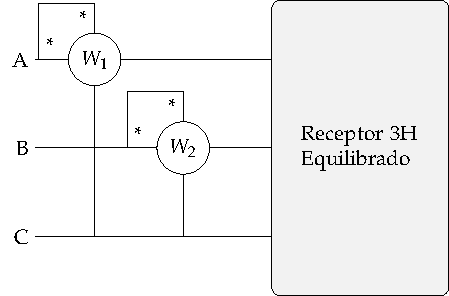
\includegraphics[width=.9\linewidth]{../figs/Potencia3H_Equilibrado_AB.pdf}
\end{center}
\end{column}

\begin{column}{0.3\columnwidth}
\begin{align*}
  W_1 &= \Re(\overline{U}_{AC} \cdot \overline{I}^*_A) = ?\\
  W_2 &= \Re(\overline{U}_{BC} \cdot \overline{I}^*_B) = ?\\
\end{align*}
\end{column}
\end{columns}
\end{frame}


\begin{frame}[label={sec:org23561de}]{Sistema de 3 Hilos Equilibrado}
Supongamos SFD:

\begin{align*}
  \overline{U}_{AC} &= - \overline{U}_{CA} = U\phase{\ang{-120} + \ang{180}} = U\phase{\ang{60}}\\
  \overline{I}_A &= I\phase{\ang{90} - \theta}\\
  \overline{U}_{AC} \cdot \overline{I}^*_A &= UI\phase{\theta - \ang{30}} \rightarrow   \boxed{W_1 = UI\cos(\theta - \ang{30})}
\end{align*}

\begin{align*}
  \overline{U}_{BC} &=  U\phase{0}\\
  \overline{I}_B &= I\phase{\ang{-30} - \theta}\\
  \overline{U}_{BC} \cdot \overline{I}^*_B &= UI\phase{\theta + \ang{30}} \rightarrow   \boxed{W_2 = UI\cos(\theta + \ang{30})}
\end{align*}
\end{frame}

\begin{frame}[label={sec:org09160bf}]{Sistema de 3 Hilos Equilibrado}
Desarrollamos los dos cosenos:
\begin{align*}
  \cos(\ang{30} - \theta) &= \cos\ang{30}\cos\theta + \sin\ang{30}\sin\theta\\
  \cos(\ang{30} + \theta) &= \cos\ang{30}\cos\theta - \sin\ang{30}\sin\theta
\end{align*}

Si sumamos obtenemos la potencia activa:
\[
  \boxed{W_1 + W_2 = \sqrt{3} U I \cos\theta = P}
\]

Si restamos obtenemos la potencia reactiva (salvo un factor):
\[
  \boxed{W_1 - W_2 = U I \sin\theta = \frac{Q}{\sqrt{3}}}
\]

Por tanto, también podemos calcular el ángulo del receptor:
\[
  \boxed{\tan\theta = \sqrt{3} \frac{W_1 - W_2}{W_1 + W_2}}
\]
\end{frame}

\begin{frame}[label={sec:org2412aae}]{Sistema de 3 Hilos Equilibrado}
Repetimos el desarrollo con SFI:

\begin{align*}
  \overline{U}_{AC} &= - \overline{U}_{CA} = U\phase{\ang{120} + \ang{180}} = U\phase{\ang{-60}}\\
  \overline{I}_A &= I\phase{\ang{-90} - \theta}\\
  \overline{U}_{AC} \cdot \overline{I}^*_A &= UI\phase{\theta + \ang{30}} \rightarrow   \boxed{W_1 = UI\cos(\theta {\color{red}+} \ang{30})}
\end{align*}
\begin{align*}
  \overline{U}_{BC} &=  U\phase{0}\\
  \overline{I}_B &= I\phase{\ang{30} - \theta}\\
  \overline{U}_{BC} \cdot \overline{I}^*_B &= UI\phase{\theta - \ang{30}} \rightarrow \boxed{W_2 = UI\cos(\theta {\color{red}-} \ang{30})}
\end{align*}
\[
  \boxed{W_1 + W_2 = \sqrt{3} U I \cos\theta = P}
\]
\[
  \boxed{W_1 - W_2 = {\color{red}-} U I \sin\theta = {\color{red}-} \frac{Q}{\sqrt{3}}}
\]
\end{frame}



\begin{frame}[label={sec:org87519c6}]{Sistema de 3 Hilos Equilibrado}
\begin{center}
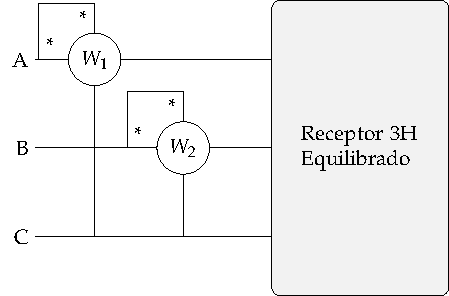
\includegraphics[height=0.3\textheight]{../figs/Potencia3H_Equilibrado_AB.pdf}
\end{center}

\begin{columns}
\begin{column}{0.5\columnwidth}
SFD
\begin{align*}
  W_1 &= UI\cos(\theta {\color{red}-} \ang{30})\\
  W_2 &= UI\cos(\theta {\color{red}+} \ang{30})
\end{align*}
\begin{align*}
  P &= W_1 + W_2\\
  Q &= \sqrt{3}({\color{red}W_1 - W_2}) \\
  \tan\theta &= \sqrt{3} \frac{{\color{red}W_1 - W_2}}{W_1 + W_2}
\end{align*}
\end{column}
\begin{column}{0.5\columnwidth}
SFI
\begin{align*}
  W_1 &= UI\cos(\theta {\color{red}+} \ang{30})\\
  W_2 &= UI\cos(\theta {\color{red}-} \ang{30})
\end{align*}
\begin{align*}
  P &= W_1 + W_2\\
  Q &= \sqrt{3}({\color{red}W_2 - W_1}) \\
  \tan\theta &= \sqrt{3} \frac{{\color{red}W_2 - W_1}}{W_1 + W_2}
\end{align*}
\end{column}
\end{columns}
\end{frame}
\begin{frame}[label={sec:org4394c89},plain]{Otras conexiones: 3H SFD}
\[
  \boxed{(ABC) :: A \triangleright B \triangleright C \Longrightarrow \{AB, BC, CA\}}
\]
\begin{align*}
  W_1 &= UI\cos(\theta - \ang{30}) & P &= W_1 + W_2\\
  W_2 &= UI\cos(\theta + \ang{30}) & Q &= \sqrt{3}(W_1 - W_2)
\end{align*}
\begin{columns}
\begin{column}{0.33\columnwidth}
\begin{center}
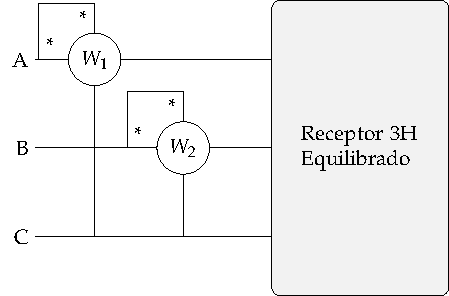
\includegraphics[width=.9\linewidth]{../figs/Potencia3H_Equilibrado_AB.pdf}
\end{center}
\begin{align*}
  W_1&: AC \notin SFD\\
  W_2&: BC \in SFD\\
\end{align*}
\end{column}
\begin{column}{0.33\columnwidth}
\begin{center}
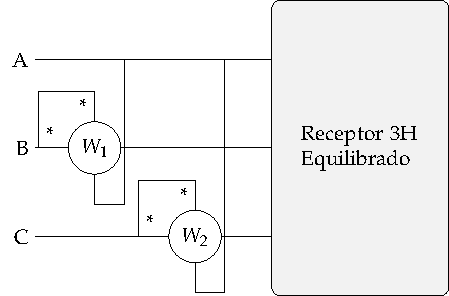
\includegraphics[width=.9\linewidth]{../figs/Potencia3H_Equilibrado_BC.pdf}
\end{center}
\begin{align*}
  W_1&: BA \notin SFD\\
  W_2&: CA \in SFD\\
\end{align*}
\end{column}

\begin{column}{0.33\columnwidth}
\begin{center}
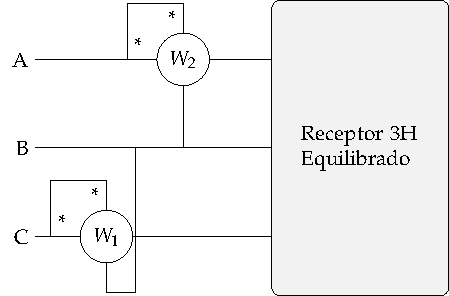
\includegraphics[width=.9\linewidth]{../figs/Potencia3H_Equilibrado_CA.pdf}
\end{center}
\begin{align*}
  W_1&: CB \notin SFD\\
  W_2&: AB \in SFD\\
\end{align*}
\end{column}
\end{columns}
\end{frame}

\begin{frame}[label={sec:orgd96ca01},plain]{Otras conexiones: 3H SFI}
\[
  \boxed{(ACB) :: A \triangleright C \triangleright B \Longrightarrow \{AC, CB, BA\}}
\]
\begin{align*}
  W_1 &= UI\cos(\theta - \ang{30}) & P &= W_1 + W_2\\
  W_2 &= UI\cos(\theta + \ang{30}) & Q &= \sqrt{3}(W_1 - W_2)
\end{align*}
\begin{columns}
\begin{column}{0.33\columnwidth}
\begin{center}
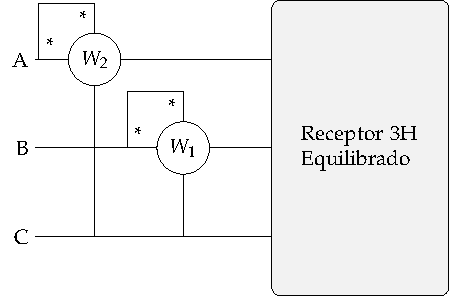
\includegraphics[width=.9\linewidth]{../figs/Potencia3H_Equilibrado_AB_SFI.pdf}
\end{center}
\begin{align*}
  W_1&: BC \notin SFI\\
  W_2&: AC \in SFI\\
\end{align*}
\end{column}
\begin{column}{0.33\columnwidth}
\begin{center}
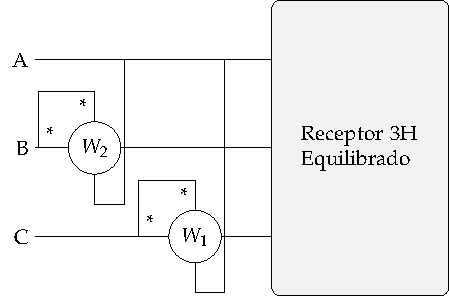
\includegraphics[width=.9\linewidth]{../figs/Potencia3H_Equilibrado_BC_SFI.pdf}
\end{center}
\begin{align*}
  W_1&: CA \notin SFI\\
  W_2&: BA \in SFI\\
\end{align*}
\end{column}

\begin{column}{0.33\columnwidth}
\begin{center}
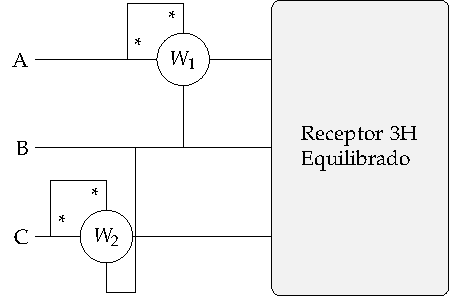
\includegraphics[width=.9\linewidth]{../figs/Potencia3H_Equilibrado_CA_SFI.pdf}
\end{center}
\begin{align*}
  W_1&: AB \notin SFI\\
  W_2&: CB \in SFI\\
\end{align*}
\end{column}
\end{columns}
\end{frame}


\begin{frame}[label={sec:org3b46001}]{Medida de Reactiva con un Vatímetro}
Cuando el sistema está equilibrado, es posible medir la potencia reactiva con un único vatímetro. 

Supongamos \alert{SFD}:

\begin{columns}
\begin{column}{0.5\columnwidth}
\begin{center}
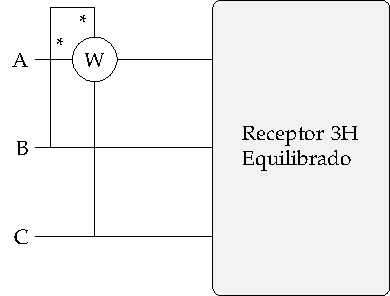
\includegraphics[width=.9\linewidth]{../figs/Reactiva3H_A-BC.pdf}
\end{center}
\end{column}

\begin{column}{0.5\columnwidth}
\[
  W = \Re(\overline{U}_{BC} \cdot \overline{I}_A^*)
\]
\begin{align*}
  \overline{U}_{BC} &= U\phase{0}\\
  \overline{I}_A &= I\phase{\ang{90} - \theta}
\end{align*}
\begin{align*}
  W &= \Re(U I \phase{\theta - \ang{90}}) = \\
    &= U I \sin(\theta)
\end{align*}
\[
  \boxed{W = \frac{Q}{\sqrt{3}}}
\]
\end{column}
\end{columns}
\end{frame}

\begin{frame}[label={sec:org3e2b3c0}]{Conexiones para medida de reactiva}
\begin{columns}
\begin{column}{0.33\columnwidth}
\begin{center}
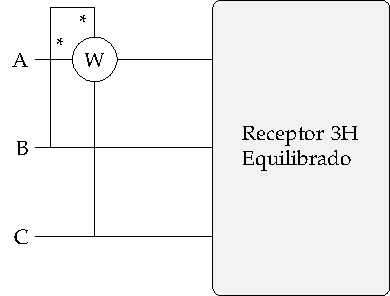
\includegraphics[height=0.25\textheight]{../figs/Reactiva3H_A-BC.pdf}
\end{center}
\[
  W = \Re(\overline{U}_{BC} \cdot \overline{I}_A^*)
\]
\begin{align*}
  BC &\in SFD\\
  BC &\notin SFI
\end{align*}
\end{column}
\begin{column}{0.33\columnwidth}
\begin{center}
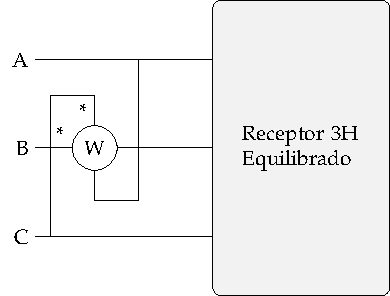
\includegraphics[height=0.25\textheight]{../figs/Reactiva3H_B-CA.pdf}
\end{center}
\[
  W = \Re(\overline{U}_{CA} \cdot \overline{I}_B^*)
\]
\begin{align*}
  CA &\in SFD\\
  CA &\notin SFI
\end{align*}
\end{column}
\begin{column}{0.33\columnwidth}
\begin{center}
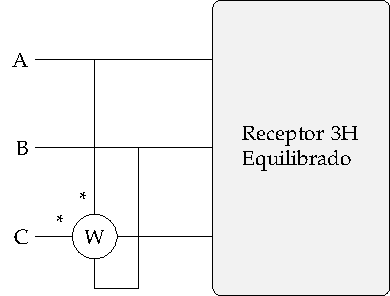
\includegraphics[height=0.25\textheight]{../figs/Reactiva3H_C-AB.pdf}
\end{center}
\[
  W = \Re(\overline{U}_{AB} \cdot \overline{I}_C^*)
\]
\begin{align*}
  AB &\in SFD\\
  AB &\notin SFI
\end{align*}
\end{column}
\end{columns}
\begin{align*}
SFD &\rightarrow \boxed{W = \frac{Q}{\sqrt{3}}}\\
SFI &\rightarrow \boxed{W =  - \frac{Q}{\sqrt{3}}}
\end{align*}
\end{frame}

\begin{frame}[label={sec:orgccc77ea}]{Conexiones para medida de reactiva}
\begin{columns}
\begin{column}{0.33\columnwidth}
\begin{center}
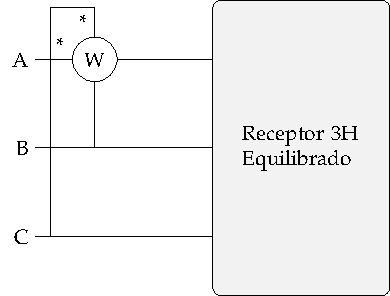
\includegraphics[height=0.25\textheight]{../figs/Reactiva3H_A-CB.pdf}
\end{center}
\[
  W = \Re(\overline{U}_{CB} \cdot \overline{I}_A^*)
\]
\begin{align*}
  CB &\notin SFD\\
  CB &\in SFI
\end{align*}
\end{column}
\begin{column}{0.33\columnwidth}
\begin{center}
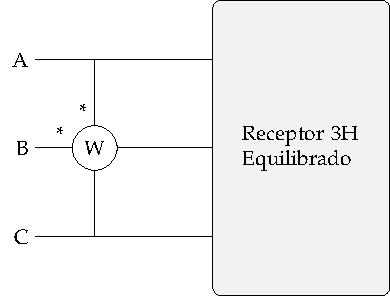
\includegraphics[height=0.25\textheight]{../figs/Reactiva3H_B-AC.pdf}
\end{center}
\[
  W = \Re(\overline{U}_{AC} \cdot \overline{I}_B^*)
\]
\begin{align*}
  AC &\notin SFD\\
  AC &\in SFI
\end{align*}
\end{column}
\begin{column}{0.33\columnwidth}
\begin{center}
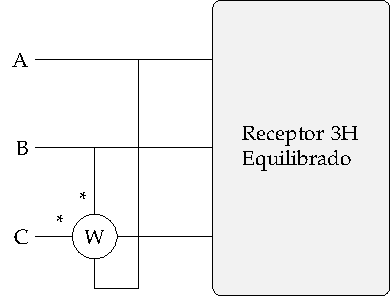
\includegraphics[height=0.25\textheight]{../figs/Reactiva3H_C-BA.pdf}
\end{center}
\[
  W = \Re(\overline{U}_{BA} \cdot \overline{I}_C^*)
\]
\begin{align*}
  BA &\notin SFD\\
  BA &\in SFI
\end{align*}
\end{column}
\end{columns}
\begin{align*}
SFD &\rightarrow \boxed{W = - \frac{Q}{\sqrt{3}}}\\
SFI &\rightarrow \boxed{W = \frac{Q}{\sqrt{3}}}
\end{align*}
\end{frame}


\subsection{Compensación de Reactiva}
\label{sec:orgcb15830}

\begin{frame}[label={sec:org1b03d63}]{Objetivo}
\begin{itemize}
\item Sea un receptor \alert{equilibrado} \alert{inductivo} del que conocemos \(P\), \(Q\) y, por tanto, su factor de potencia \(\cos \theta\).

\item Para reducir la potencia reactiva del sistema debemos instalar un \alert{banco de condensadores} que suministrarán una potencia reactiva \(Q_c\).

\item Como \alert{resultado}, la potencia reactiva y el factor de potencia del sistema serán \(Q' = Q - Q_c\) y \(\cos\theta' > \cos \theta\).

\item En trifásica existen dos posibilidades:
\begin{itemize}
\item Conexión en triángulo: \(C_\triangle\)
\item Conexión en estrella: \(C_Y\).
\end{itemize}
\end{itemize}
\end{frame}

\begin{frame}[label={sec:orgde4e6f1}]{Conexión en Triángulo}
\begin{columns}
\begin{column}{0.5\columnwidth}
\begin{center}
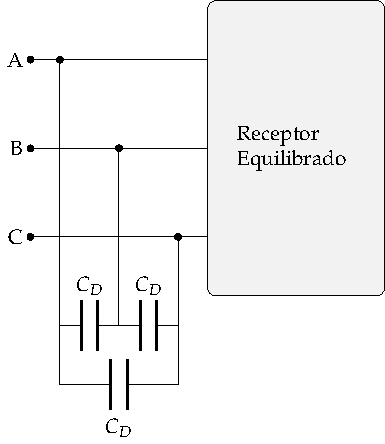
\includegraphics[width=.9\linewidth]{../figs/CircuitoTrifasica_CompensacionReactiva.pdf}
\end{center}
\end{column}

\begin{column}{0.5\columnwidth}
\begin{align*}
  Q &= P\tan\theta\\
  Q' &= P\tan\theta' =\\
    &= Q - Q_c\\
  Q_c &= 3 \cdot \omega C_\triangle \cdot U^2
\end{align*}
\[
  \boxed{C_\triangle = \frac{P(\tan \theta - \tan \theta')}{3\omega U^2}}
\]
\end{column}
\end{columns}
\end{frame}

\begin{frame}[label={sec:orga7ba61e}]{Conexión en Estrella}
\begin{columns}
\begin{column}{0.5\columnwidth}
\begin{center}
\includegraphics[width=.9\linewidth]{../figs/CircuitoTrifasicaY_CompensacionReactiva.pdf}
\end{center}
\end{column}
\begin{column}{0.5\columnwidth}
\begin{align*}
  Q &= P\tan\theta\\
  Q' &= P\tan\theta' =\\
    &= Q - Q_c\\
  Q_c &= 3 \cdot \omega C_Y \cdot U_f^2
\end{align*}
\[
  \boxed{C_Y = \frac{P(\tan \theta - \tan \theta')}{\omega U^2}}
\]
\end{column}
\end{columns}
\end{frame}
\begin{frame}[label={sec:org28560b8}]{Comparación Estrella-Triángulo}
\begin{columns}
\begin{column}{0.5\columnwidth}
\begin{center}
\includegraphics[height=0.55\textheight]{../figs/CircuitoTrifasica_CompensacionReactiva.pdf}
\end{center}
\[
  \boxed{C_\triangle = \frac{P(\tan \theta - \tan \theta')}{3 \omega U^2}}
\]
\end{column}

\begin{column}{0.5\columnwidth}
\begin{center}
\includegraphics[height=0.55\textheight]{../figs/CircuitoTrifasicaY_CompensacionReactiva.pdf}
\end{center}
\[
  \boxed{C_Y = \frac{P(\tan \theta - \tan \theta')}{\omega U^2}}
\]

\medskip
\end{column}
\end{columns}

Dado que \(C_Y = 3 \cdot C_\triangle\) la \alert{configuración recomendada} es \alert{triángulo}.
\end{frame}
\subsection{Comparativa Monofásica-Trifásica}
\label{sec:org776f8fb}

\begin{frame}[label={sec:org012a779}]{Potencia Instantánea en Sistemas Equilibrados}
Supongamos un receptor equilibrado en estrella con SFD:

\begin{columns}
\begin{column}{0.5\columnwidth}
\begin{align*}
  u_A(t) &= \sqrt{2} U_f \cos(\omega t + \ang{90})\\
  u_B(t) &= \sqrt{2} U_f \cos(\omega t - \ang{30})\\
  u_C(t) &= \sqrt{2} U_f \cos(\omega t - \ang{150})
\end{align*}

\begin{align*}
  i_A(t) &= \sqrt{2} I \cos(\omega t + \ang{90} - \theta)\\
  i_B(t) &= \sqrt{2} I \cos(\omega t - \ang{30} - \theta)\\
  i_C(t) &= \sqrt{2} I \cos(\omega t - \ang{150} - \theta)
\end{align*}
\end{column}

\begin{column}{0.5\columnwidth}
\begin{align*}
  p_A(t) &= u_A(t) \cdot i_A(t)\\
  p_B(t) &= u_B(t) \cdot i_B(t)\\
  p_C(t) &= u_C(t) \cdot i_C(t)\\
  \\
  p(t) &= p_A(t) + p_B(t) + p_C(t)
\end{align*}
\end{column}
\end{columns}
\end{frame}

\begin{frame}[label={sec:org9ed8f04}]{Potencia Instantánea en Sistemas Equilibrados}
\begin{align*}
  p(t) &= \sqrt{2}U_f  \cos(\omega t + \ang{90}) \cdot \sqrt{2}I\cos(\omega t + \ang{90} - \theta) +\\
       &+ \sqrt{2}U_f \cos(\omega t - \ang{30}) \cdot \sqrt{2}I \cos(\omega t - \ang{30} - \theta) +\\
       &+ \sqrt{2}U_f \cos(\omega t - \ang{150}) \cdot \sqrt{2}I \cos(\omega t - \ang{150} - \theta)
\end{align*}
\[
  \cos(\alpha) \cdot \cos(\beta) = \frac{1}{2} \cdot (\cos(\alpha + \beta) + \cos(\alpha - \beta))
\]
\begin{align*}
  p(t) &= U_f I [{\color{gray}\cos(2 \omega t + \ang{180} -\theta)} + \cos(\theta)] +\\
       &+ U_f I [{\color{gray}\cos(2 \omega t - \ang{60} - \theta)} + \cos(\theta)] +\\
       &+ U_f I [{\color{gray}\cos(2 \omega t - \ang{300} - \theta)} + \cos(\theta)]
\end{align*}
\[
  \boxed{p(t) = 3 \cdot U_f \cdot I \cdot \cos (\theta) = \sqrt{3} \cdot U \cdot I \cdot \cos (\theta)} 
\]
\end{frame}


\begin{frame}[label={sec:orgb763435}]{Masa de conductor}
Comparemos un sistema monofásico y un sistema trifásico (3H) que transmiten la \alert{misma potencia activa} y funcionan a la \alert{misma tensión entre líneas}.
\[
U I_1 \cos\theta = P_1 = P_3 = \sqrt{3}U I_3 \cos\theta \rightarrow \boxed{I_1 = \sqrt{3} I_3}
\]
Las \alert{pérdidas en la línea} deben ser \alert{iguales} para salvar la \alert{misma distancia}:
\[
  2R_1I_1^2 = P_{1l} = P_{3l} = 3R_3I_3^2
\]
Sustituyendo la relación de corrientes y teniendo en cuenta la relación entre resistencia y sección:
\[
  2\cdot R_1 \cdot 3I_3^2 = 3\cdot R_3 I_3^2 \rightarrow R_1 = \frac{1}{2} R_3 \rightarrow \boxed{S_1 = 2 \cdot S_3}
\]

Finalmente, la relación entre masas de conductor es:

\[
  \frac{m_3}{m_1} = \frac{3 \cdot S_3}{2 \cdot S_1} = \boxed{\frac{3}{4}}
\]
\end{frame}
\end{document}